\documentclass[aps, prc, reprint, amsmath, groupedaddress, nofootinbib]{revtex4-1}
%\usepackage[compat=1.1.0]{tikz-feynman}
\usepackage[utf8]{inputenc}
\usepackage{hyperref}
\usepackage{amsmath}
\usepackage{amssymb}
\usepackage{amsfonts}
\usepackage{tabularx}
\usepackage{booktabs}
\usepackage{graphicx}
\usepackage{color}
\usepackage{multirow}
\usepackage{verbatim}
\usepackage[inline]{enumitem}
\graphicspath{{fig/}}
\definecolor{theblue}{RGB}{0,50,230}
\usepackage{appendix}
\hypersetup{
  colorlinks=true,
  linkcolor=theblue,
  citecolor=theblue,
  urlcolor=theblue
} 
\usepackage[most]{tcolorbox}

\begin{abstract}
Highly energetic partons  created in perturbative processes at the onset of relativistic heavy-ion collisions  are excellent probes for the study of hot and dense deconfined QCD matter. This is accomplished by relating the energy-loss these partons suffer to the properties of the medium they traverse.
Monte-Carlo event generators, that allow for the realistic description of fluctuating initial conditions and medium properties, have become a powerful tool in this endeavor. However, the implementation of quantum coherence effects, such as the Landau-Pomeranchuk-Migdal (LPM) effect, poses a serious challenge to this class of models, since multiple interactions with the medium cannot be factorized into independent processes. 
In this work, we discuss several common implementations of the LPM effect in Monte-Carlo event generators and compare them to limiting cases in jet energy-loss theory for which semi-analytic calculations exist. We propose an approach, dubbed
``modified rescattering", that reproduces the limiting semi-analytic calculations of radiative parton energy loss for infinite and thin media  and reasonably describes gluon emission spectra. We study the impact of an expanding medium, a running coupling and heavy quark masses in this approach. 
\end{abstract}

\begin{document}
\title{Modeling of quantum-coherence effects in parton radiative energy loss}
\author{Weiyao Ke}
\author{Yingru Xu}
\author{Steffen A.\ Bass}
\affiliation{Department of Physics, Duke University, Durham, NC 27708-0305}
\date{\today}
\maketitle 

\section{Introduction}
The study of hard probes in relativistic heavy-ion collisions is moving towards the precision era thanks to upcoming experimental upgrades \cite{ATLAS-Collaboration:2012iwa,Abelevetal:2014dna,STAR:upgrade-hf,Adare:2015kwa,CMS:2017dec} as well as theoretical and computational advances that allow for the execution of jet energy-loss calculations in a realistic Quark-Gluon-Plasma (QGP) medium (including event-by-event fluctuating initial conditions and temperature-dependent transport coefficients) \cite{Wang:1994fx,Zakharov:1996fv,Baier:1996sk,Zakharov:1997uu,Arnold:2002zm,Gyulassy:2003mc,Kovner:2003zj,CasalderreySolana:2007pr,Bass:2008rv,Schenke:2009gb,Majumder:2009zu,Majumder:2010qh,Armesto:2011ht,Zapp:2011ya,Ovanesyan:2011xy,Kang:2014xsa,Cao:2016gvr,Kauder:2018cdt,Cao:2017zih}. Among the goals for this research is the characterization of the QGP medium in terms of its jet transport coefficients $\hat{q}$.

Monte-Carlo event generators are powerful tools that allow for the realistic description of fluctuating initial conditions and medium properties. 
However, the numerical implementation of quantum coherence effects, such as the Landau-Pomeranchuk-Migdal (LPM) effect, poses a serious challenge to this class of models, because coherent multiple interactions cannot be factorized into independent scatterings with the medium. 
In a dense medium, the LPM effect is important for the treatment of radiative energy-loss, which is the dominant contribution to energy-loss of partons traversing the QGP at high momentum.
Here, multiple scatterings during the gluon formation time act coherently to suppress the radiation spectrum \cite{PhysRev.103.1811,Wang:1994fx,Zakharov:1996fv,Zakharov:1997uu,Baier:1996kr,Baier:1996sk}.
Therefore, a medium induced radiation becomes effectively an $n$-body to $(n+1)$-body process that extends in space-time.
This feature is particularly difficult to accurately implement in a Monte-Carlo approach, where interactions are usually based on few-body processes that are local.
To simplify the problem while still retaining essential qualitative features such as the characteristic emission spectrum and path-length dependence of the energy loss, different methods have been used in numerical simulations \cite{Djordjevic:2008iz,Cao:2013ita,ColemanSmith:2012vr,Xu:2004mz,Zapp:2011ya,Gossiaux:2012cv,Park:thesis}.
In this work we compare three of the most common implementations based on different approximations of radiative processes to perturbative kinetic theory predictions in idealized limits \cite{Arnold:2002zm,Arnold:2008zu,Arnold:2009mr,Baier:1996kr,Baier:1998yf}. 
As we shall see, a modified approach based on the method of \cite{Zapp:2011ya} works remarkably well.
This method, referred to as the ``modified rescattering" approach, reproduces analytic calculations of energy loss as a function of coupling constant, temperature, parton energy and path length.
It also reasonably well describes the gluon radiation spectra in both static and expanding media.
We introduce parameters to control its finite- and infinite-size behaviors separately.
The parameters can be fine-tuned to match the theory or be calibrated to experimental data;
therefore, the performance of the theory can be measured quantitatively on the landscape of this parameter space in a future statistical analysis.

This paper is organized as follows. Section \ref{section:qual} reviews the qualitative spectrum of the medium induced radiation.
In Section \ref{section:MC}, three Monte Carlo implementations of radiative processes are discussed. 
Semi-analytic results to which the Monte Carlo simulations are compared are briefly summarized in Section \ref{section:Theo}.
Major results are shown in Section \ref{section:results}.
Finally, we discuss in Section \ref{section:disscuss} effects induced by the running of the coupling constant, the expanding medium and heavy quark masses (dead-cone effect) in the ``modified rescattering" implementation. We summarize in Section \ref{section:summary}.

\section{Qualitative features of the medium induced radiation}\label{section:qual}
In this section, we discuss qualitative features of medium induced radiation following the discussion in \cite{Baier:1996kr}.
A radiated gluon stays in coherence with its emitting mother parton for a finite amount of time determined by the uncertainty principle $\Delta t \sim 1/\Delta E$. 
$\Delta E$ is the difference in light-cone energy between the initial mother parton and the final state of daughter partons.
The formation time is then,
\begin{eqnarray}\label{eq:tau_1}
\tau_f \sim \frac{2(1-x)\omega}{k_\perp^2+(1-x)m_g^2}.
\end{eqnarray}
$x = \omega/E$ is the energy fraction carried by the gluon. 
$m_g^2$ is the gluon thermal mass squared which is related to the Debye screening mass by $m_g^2 = m_D^2/2 \sim \alpha_s T^2$.
For a collinear splitting, the formation time is proportional to $\omega/(\alpha_s T^2)$ .
Meanwhile, the gluon can keep interacting with the dense medium via elastic scatterings with a rate $R_{g}$ that scales like $\alpha_s T$. 
Therefore, the number of gluon rescatterings within the formation time $N \sim \tau_f R_g \sim \omega/T$ may not be a small number for gluons with energy comparable to or larger than the medium temperature.
Moreover, because rescatterings also change the transverse momentum $k_\perp$ of the gluon relative to the mother parton, a self-consistent formation time estimation is required.
Given that on average elastic scattering increases $k_\perp^2$ by an amount $\hat{q}_g\tau_f$ where $\hat{q}_g = d\langle k_\perp^2\rangle/dt$ is the gluon transport coefficient, the self-consistent relation for an averaged formation time is,
\begin{eqnarray}\label{eq:tau_n}
\tau_f \sim \frac{2(1-x)\omega}{\hat{q}_g\tau_f} \longrightarrow \tau_f \sim \sqrt{\frac{2(1-x)\omega}{\hat{q}_g}}
\end{eqnarray}
The inverse of the formation time measures the rate of a gluon being separated from the mother parton.

The radiation spectrum is understood as follows. 
A virtual gluon with energy $\omega$ and transverse momentum $k_\perp$ splits from the mother parton with a probability given by the splitting function ($P(x) \sim \alpha_s/x$).
If its formation time is smaller than the mean-free-path of elastic scattering $\lambda_g = 1/R_g$, it is put on shell with the rate $1/\lambda_g$ (the Bethe-Heitler region); otherwise multiple rescatterings put it on-shell with a rate $1/\tau_f$ (the LPM region).
As a result, the differential radiation rate is,
\begin{eqnarray}\label{eq:LPM}
\frac{dP}{dt d\omega} \sim \begin{cases}
 \frac{\alpha_s}{\omega} \frac{1}{\lambda_g} \sim \alpha_s^2  \frac{T}{\omega}, \hfill \tau_f \lesssim \lambda_g\\
 \frac{\alpha_s}{\omega} \frac{1}{\tau_f}\sim \alpha_s \sqrt{\hat{q}_g/T^3} \left(\frac{T}{\omega}\right)^{3/2}, \hfill \lambda_g \lesssim \tau_f
\end{cases}
\end{eqnarray}
We note that in the leading order picture, the LPM effect modifies the single gluon emission rate. 
It does not introduce correlations between subsequent emissions which are higher order effects \cite{Arnold:2016jnq}.
Second, the emission rate at a certain time receives coherent contributions from the collision centers whose locations extend about $\tau_f$ along the path of the mother parton.
Therefore, if the number of scattering centers in a thin medium of size $\lambda_g < L< \tau_{f,\textrm{max}} \sim \sqrt{E/\hat{q}_g}$ are limited, the second line of Equation \ref{eq:LPM} is replaced by,
\begin{eqnarray}
\frac{dP}{dt d\omega} \sim 
 \frac{\alpha_s}{\omega} \frac{1}{\min\{\tau_f,L\}}, \hfill \lambda_g < \tau_f
\end{eqnarray}
The radiative energy loss is obtained by integrating over the differential rate times the gluon energy. 
For the case of an infinite medium, this is
\begin{eqnarray}\label{eq:dE-Linf}
\Delta E/\Delta L \sim \alpha_s^2 \sqrt{ET^3}
\end{eqnarray}
Therefore for high energy patrons, the amount of energy loss is significantly reduced compared to the incoherent calculation $\Delta E/\Delta L \sim \alpha_s^2 E T$.
For a thin medium, the LPM effect leads to a non-linear path length $L$ dependence of the energy loss
\begin{eqnarray}\label{eq:dE-Lfinite}
\Delta E \sim \alpha_s \hat{q} L^2
\end{eqnarray}
When the path length exceeds the $\tau_{f,\textrm{max}}$, $\Delta E$ should smoothly transit to the behavior given by Equation \ref{eq:dE-Linf}.

\section{Comparison of Monte-Carlo implementations of the LPM effect}\label{section:MC}
In this section we compare different approaches to implementing the LPM effect in jet energy-loss transport models, focusing on those approaches that treat this effect non-locally resulting in a path length dependent emission spectrum.
The framework for our study is the {\tt Lido} model \cite{Ke:2018tsh}. 
This model was originally designed for modeling  heavy quark transport inside a QGP. 
In this work, we remove all quark mass effects (phase-space, matrix-elements) to adapt {\tt Lido} for the  study of  light quark energy-loss.
The {\tt Lido} model is based on elementary ($2\rightarrow2$) elastic and inelastic pQCD scatterings. 
The inelastic processes include both gluon radiation ($2\rightarrow 3$) and gluon absorption ($3\rightarrow 2$) processes using an improved Gunion-Bertsch approximated matrix-element \cite{Fochler:2013epa,Uphoff:2014hza}.

%\begin{tcolorbox}[width=\columnwidth]
We modify the original {\tt Lido} diffusion plus scattering setup by introducing a momentum transfer ($\hat{t}$) separation scale $\hat{t}_{\textrm{cut}}$. 
Large-angle $2\rightarrow 2$ elastic scatterings ($|\hat{t}| > \hat{t}_{\textrm{cut}}$) and associated $2\rightarrow 3$ inelastic scatterings are solved by a rate equation while small-angle ($|\hat{t}| < \hat{t}_{\textrm{cut}}$) processes are solved by a diffusion equation with diffusion induced radiation. 
Accordingly, the pQCD transport coefficient for the diffusion equation is  calculated by integrating the collision kernel $\mathcal{A}(q^2)$ (Equation \ref{eq:kernel} ) upto the separation scale, denoted as $\hat{q}_{<}$
\begin{eqnarray}
\hat{q}_{<} = \alpha_s C_R \int_0^{\hat{t}_{\textrm{cut}}} \mathcal{A}(q^2) q^2 dq^2.
\end{eqnarray}
Choosing a reasonable value of $gT < \hat{t}_{\textrm{cut}} < T$, this decomposition is shown to be equivalent to the leading order transport equation \cite{Ghiglieri:2015ala}.
However, the new decomposition has a number of advantages: first, the model is not plagued by a rate that diverges when $\hat{t} \rightarrow 0$.
Second, the pure diffusion plus induced radiation model is nested as a limiting case by choosing $\hat{t}_{\textrm{cut}}\rightarrow \infty$.
Third, one can utilize a parametric form of correction to $\hat{q}_{<}$ and extract it from a model-to-data calibration.
%\end{tcolorbox}

For the purpose of comparing different MC implementations of LPM suppression to theory calculations, we focus on the $2\rightarrow 3$ channel for the highly energetic quark and the $t$-channel for the elastic scatterings.
Next, we introduce three different LPM effect implementations in detail.

\paragraph*{``Coherence factor" approach} This first approach is the one previously used in the {\tt Lido} model. 
It is similar to the higher-twist formula used in the radiation improved Langevin equation \cite{Cao:2013ita} and the Linearized-Boltzmann-Transport-Model \cite{Cao:2016gvr,Cao:2017hhk}.
In the {\tt Lido} model, we start from the incoherent rate of a $2\rightarrow 3$ process using the Gunion-Bertsch cross-section $\sigma_\textrm{GB}$,
\begin{eqnarray}\label{eq:GB-rate}
\Gamma = \frac{1}{2E_1}\int\frac{f_i(p_2)d\vec{p_2}^3}{(2\pi)^3 2p_2}2\hat{s}\int d\hat{t}\frac{d\vec{k}^3}{(2\pi)^3 2k}\frac{d\sigma_{\textrm{GB}}}{d\hat{t}d\vec{k}^3}.
\end{eqnarray}
The ``Coherence factor" approach implements LPM suppression by multiplying a time-dependent coherence factor to the final state gluon phase space integration in Equation \ref{eq:GB-rate},
\begin{eqnarray}\label{eq:GB-rate-LPM}
\frac{d\vec{k}^3}{(2\pi)^3 2k} \rightarrow \frac{d\vec{k}^3}{(2\pi)^3 2k} 2\left[1-\cos\left(\frac{t-t_0}{\tau_f}\right)\right].
\end{eqnarray}
The modified rate depends on the time separation $\Delta t = t-t_0$ which is the time elapsed from the last gluon emission.
Performing the small angle scattering approximation to the Gunion-Bertsch matrix-element (please refer to Appendix \ref{app:consistency} for details), the Gunion-Bertsch rate can be rewritten into a diffusion induced radiation rate
\begin{eqnarray}\label{eq:GB-small-angle-rate}
\Gamma = \hat{q}_g\int\frac{\alpha_s}{\pi}\frac{C_F dx}{x} \frac{dk_\perp^2}{k_\perp^4}.
\end{eqnarray}
This would be the same as the one used in \cite{Cao:2013ita} if the coherence factor is included.
The value of $\Delta t$ is only determined at run-time,
but its order-of-magnitude can still be estimated  from the following condition:
\begin{eqnarray}\label{eq:delta-t-1}
\nonumber
1 &\sim& \int_0^{\Delta t}\Gamma(t) dt,\\
&=& \Delta t \int d\Gamma \left[1-\frac{\sin(\Delta t/\tau_f)}{\Delta t/\tau_f}\right],
\end{eqnarray}
which implies that the probability to have one radiation within $\Delta t$ should be of order $1$ required by the definition of $\Delta t$.
A dimensional analysis (Appendix \ref{app:consistency}) shows $\Delta t \sim 1/\alpha_s T$.
We see that this prescription indeed suppresses the spectrum when the formation time is much longer than the mean-free-path. 
However, multiple scatterings are not included in this approach since gluons are always produced in $2\rightarrow3$ processes.
Moreover, this approach introduces a correlation between the locations of vertices of subsequent emissions;
especially, no matter how soft the previous radiation is, it always affects the next radiation and the prediction depends on the minimum gluon energy cut-off in a logarithmic fashion.

The next two approaches both include multiple scatterings  during the formation time determination based on a method motivated by \cite{Zapp:2011ya}.
A gluon is first sampled from a $2\rightarrow3$ inelastic scattering at time $t=t_0$, but it is not immediately regarded as ``formed". 
This gluon may keep interacting with the medium via elastic processes. The gluon transverse momentum $k_{\perp,n}$ and formation time $\tau_{f,n}$ is modified after each rescattering.
Here, the subscripts $n$ denote the quantities calculated after the $n$-th rescattering.
This continues until the time elapsed since $t_0$ exceeds the gluon formation time after the $n$-th rescattering,
\begin{eqnarray}\label{eq:self-consisten-condition}
\tau_{f, n} < t-t_0 < \tau_{f, n-1}.
\end{eqnarray}
At that time, the gluon is considered to have lost coherence with its mother parton.
The formation time determined in this way fulfills the self-consistent condition of Equation \ref{eq:tau_n}.
Using the self-consistent formation time, we find that there are at least two ways to introduce suppression. In this work, we discuss the following two approaches and discuss their validity:

\paragraph*{``Block radiation" approach}
In this approach, LPM suppression is introduced by requiring that no other radiation is allowed within $t-t_0$ shown in Equation \ref{eq:self-consisten-condition}.
A similar method is employed in \cite{ColemanSmith:2012vr}.
This approach suppresses the radiation rate and also results in a non-linear path length dependence of the energy loss. However, a closer examination reveals a number of shortcomings: 
First of all, the approach again introduces correlations between subsequent emission vertices.
Secondly, it does not alter the shape of the radiation spectrum. Even though each branching is delayed by $\tau_f$, it is still generated according to the incoherent differential probability. 
The $2\rightarrow 3$ spectrum is only suppressed by an overall factor $1/N$ that reduces $N$ possible inelastic collisions to a single one,
\begin{eqnarray}
N \sim \frac{\left\langle\tau_{f,N}\right\rangle}{ \lambda_{\textrm{inel}}}.
\end{eqnarray}
This is different from the expected qualitative behavior, since $\lambda_{\textrm{inel}}$ is used instead of the correct usage of $\lambda_{\textrm{el}}$.
This approach certainly does not reproduce the desired limits -- we retain it in our comparison as an instructive example.

\paragraph*{``Modified rescattering" approach} This  approach (which we shall adopt as the default for {\tt Lido} moving forward) is a  modification of the one studied in \cite{Zapp:2011ya,Park:thesis,Park:2016jap}.


For our discussion we define an ``effective" mean-free-path $\tilde{\lambda}$,
\begin{eqnarray}\label{eq:effmpf}
\tilde{\lambda} = \frac{m_D^2}{\hat{q}_g(\omega, T)}.
\end{eqnarray}
Unlike the mean-free-path that may be sensitive to the regulator, it only relates to well defined quantities and can also be used in models using a diffusion approximation for elastic processes so long as $\hat{q}$ is given.


Another change is the redefinition of the gluon formation time off a quark,
\begin{eqnarray}\label{eq:formation-time-def}
\tau_f = \frac{2(1-x)\omega}{\left(1-x+C_F/C_A x^2\right)k_\perp^2 + (1-x)m_g^2}.
\end{eqnarray}
The additional factor in front of $k_\perp^2$ is motivated by the semi-analytic calculation to be discussed in the next section. It is due to the system under consideration consisting not only of a gluon but also the mother quark and the other daughter parton. 
This factor reduces to unity in the soft limit $x\ll 1$, but it increases the formation time for harder splittings. 

With these building blocks, we present the following step-by-step implementation,
\begin{itemize}
\item[1.] Within $\Delta t$, a mother parton undergoes both large-angle inelastic scattering and diffusion induced radiation with rates from Equations \ref{eq:GB-rate} and \ref{eq:GB-small-angle-rate}.
\item[2.] If a gluon $i$ is sampled at $t_{i,0}$, it is appended to a ``pre-formed gluons" list associated with the mother parton. But its energy is not carried away.
\item[3.] Loop over the ``pre-formed gluons" list. 
\begin{itemize}
\item[3.1] If $\tau_f > t-t_{i,0}$, evolve this gluon by both large-angle elastic scatterings and small-angle diffusion. Recalculate its formation time.
\item[3.2] If $\tau_f < t-t_{i,0}$, accept it with probability $p = \min\{1, u\tilde{\lambda}/\tau_f\}$. Accepted gluons are formed and their energies are subtracted from the mother. Otherwise, they are removed from the list without causing energy loss.
\end{itemize} 
\item[4.] Repeat for the next time step.
\end{itemize}
Here, we use the term ``pre-formed gluons" to denote those gluons that stay in coherence with the mother parton.
A parton may carry an arbitrary number of ``pre-formed gluons" and there are no correlations among them.
The formation time calculated after multiple scatterings scales like $\sqrt{\omega/\hat{q}}$ on average, so the factor $\tilde{\lambda}/\tau_f$ guarantees that the radiation spectra in the LPM region scales like the qualitative one in Equation \ref{eq:LPM}.
Next we discuss the significance of the factor $u$:
We first point out that the formation time from the above procedure is only valid to leading-log level.
In a Monte-Carlo simulation, the final transverse momenta $k_\perp^2\sim \tau_f \hat{q} \sim \tau_f \alpha_s^2 T^3 \ln(Q_0^2/m_D^2)$, 
and $Q_0^2\sim \hat{s}$ is the maximum momentum transfer squared in each elastic scattering.
However, from a total coherent point of view, these re-scatterings act like a single one except that the maximum $Q_0^2$ should be of the order of $k_\perp^2 = \tau_f \hat{q}$.
Therefore, there is a mismatch in the argument of the logarithm.
The $u$ term is introduced to correct for this mismatch,
\begin{eqnarray}
u &=& \left\{\frac{\ln\left(1+\frac{\tau_f\hat{q}}{m_D^2}\right)}{\ln\left(1+\frac{\hat{s}}{m_D^2}\right)}\right\}^{\frac{1}{2}}
\approx \left\{\frac{\ln\left(1+\tau_f/\tilde{\lambda}\right)}{\ln\left(1+\frac{6\omega T}{m_D^2}\right)}\right\}^{\frac{1}{2}},
\end{eqnarray} 
where we have used $\left\langle\hat{s}\right\rangle \approx 6 \omega T$.
This is also motivated by the next-to-leading-log approximation in the AMY formalism discussed in the next section.

Finally, we point out that Equations \ref{eq:effmpf} and \ref{eq:formation-time-def} only encode the scaling of these quantities, so in practice we introduce the following tunable relations,
\begin{eqnarray}\label{eq:tune}
\nonumber
\tau_f & \rightarrow & C_1 \tau_f, \\
\tilde{\lambda} & \rightarrow & C_2 \tilde{\lambda}.
\end{eqnarray}
The parameters $C_1$ and $C_2$ are unity by default and control the finite- and infinite-size behaviors respectively. 
This is possible by realizing that in this algorithm the comparison between medium length and the formation time solely determines the finite size scaling; while the acceptance criterion alone controls the magnitude of suppression.
Though it is possible to fine-tune these parameters systematically, we will show that the default $C_1 = 1, C_2 = 1$ already works very well.

%Finally, we point out that those ``pre-gluons" in this approach do not have to be medium induced from the very beginning. 
%Gluons from the vaccum shower of a hard parton generated by, {\tt Pythia} e.g., can also be initialized as ``pre-gluons" associated to the hard parton to study the interplay between the vacuum shower and the medium effect.
%Of course this is already out of the scope of the current paper.

\section{Semi-analytic reference calculation}\label{section:Theo}
The full leading-order calculation of parton radiative energy-loss in a ``brick" medium and the comparison between different approximations has been discussed in detail in \cite{CaronHuot:2010bp}.
Due to the complexity of the full calculation, we only quote its numerical results for the radiation spectra in a finite medium.
For other comparisons in a static medium, we make use of two (semi-)analytic results where medium induced gluon radiation is solved in an infinitely large medium (to next-to-leading-log accuracy) \cite{Arnold:2008zu} and in a thin medium (to leading-log accuracy) \cite{Arnold:2009mr}.
We also utilize a calculation performed in an expanding medium \cite{Baier:1998yf}, as it is much closer to the reality in heavy-ion collisions than the static approximations.
For the reader's convenience, we briefly summarize the formula borrowed from \cite{Arnold:2008zu,Arnold:2009mr,Baier:1998yf} in this section.

\begin{figure*}
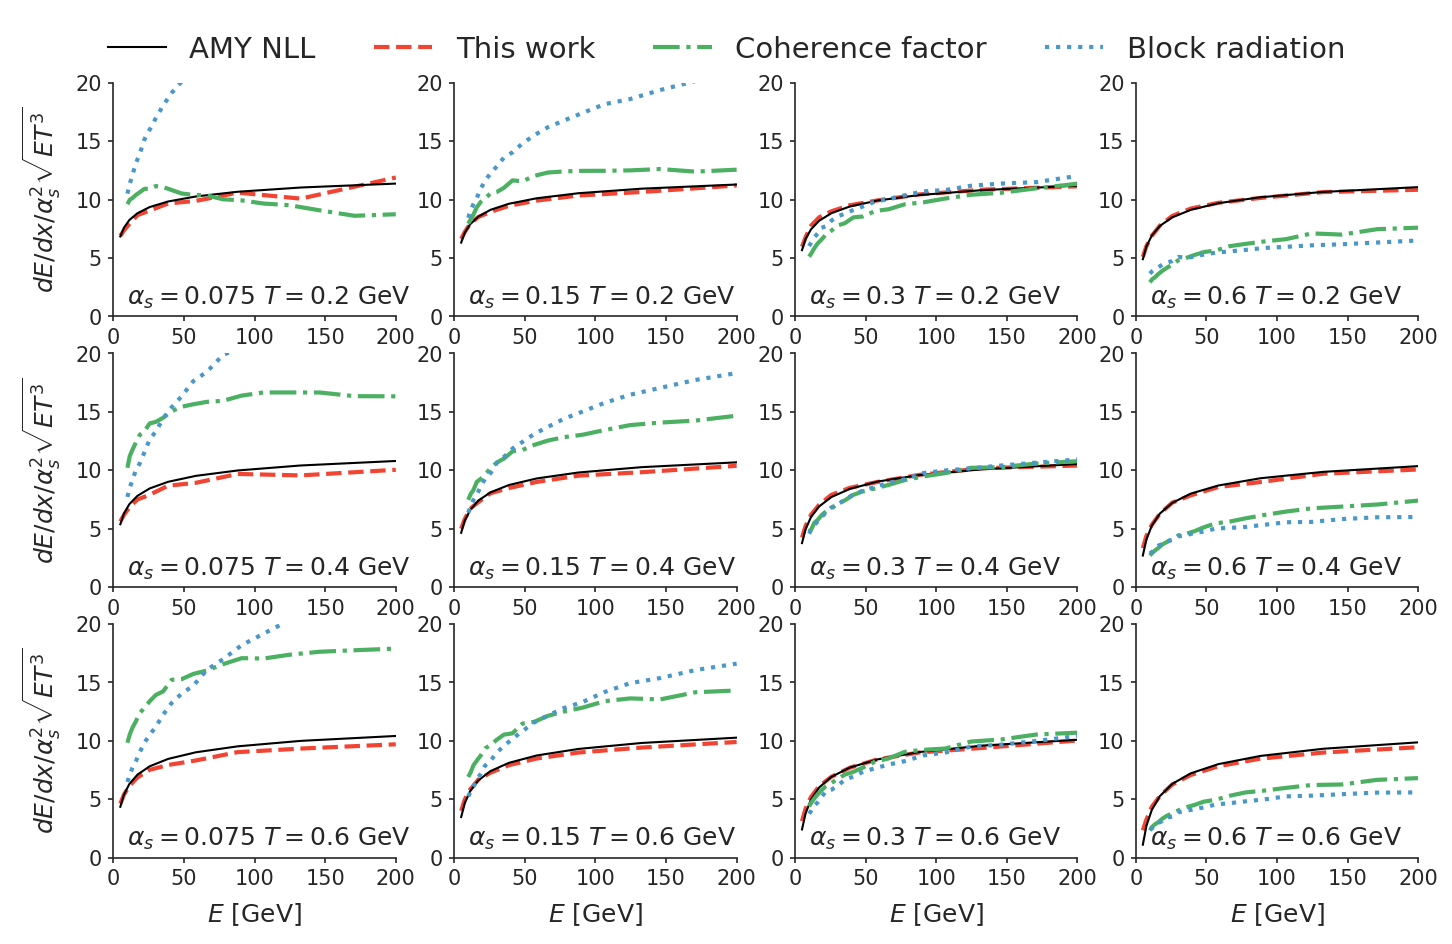
\includegraphics[width=\textwidth]{Eloss_infinite.png}
\caption{Energy loss per unit path lengh $dE/dx$ as a function of energy $E$, temperature $T$ and coupling constant $\alpha_s$. Each column corresponds to a value of the coupling constant $\alpha_s = 0.075, 0.15, 0.3$, and $0.6$ (from left to right). Each row corresponds to a temperature of $T = 0.2, 0.4$, and $0.6$ GeV (from top to bottom). $dE/dx$ is divided by the expected scaling $\alpha_s^2 \sqrt{ET^3}$. The MC implementations of the LPM effect referred to as ``modified rescattering", ``coherence factor", and ``block radiation" approaches are shown with red-dashed lines, blue-dash-dotted lines, and green-dotted lines respectively. The AMY NLL results are denoted as black boxes.}
\label{fig:eloss-inf}
\end{figure*}

\begin{figure*}
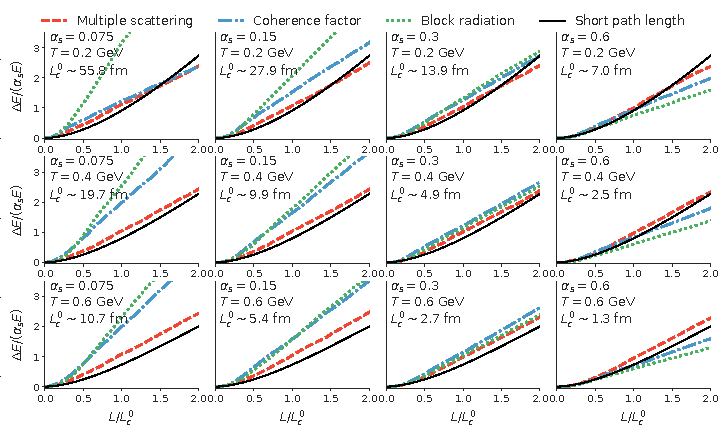
\includegraphics[width=\textwidth]{Eloss_Ldep.png}
\caption{Energy loss $\Delta E$ as a function of path length $L$, temperature $T$ and coupling constant $\alpha_s$. Each column corresponds to a coupling constant of value $\alpha_s = 0.075, 0.15, 0.3$, and $0.6$ (from left to right). Each row corresponds to a temperature of value $T = 0.2, 0.4$, and $0.6$ GeV (from top to bottom). $\Delta E$ is scaled by $\alpha_s E$ and $L$ is scaled by an estimated critical path length $L_c^0 = \sqrt{E/\hat{q}_0}$, $\hat{q}_0 = C_A \alpha_s T m_D^2$. The MC implementations of the LPM effect referred to as ``modified rescattering", ``coherence factor", and ``block radiation" approaches are the red-dashed lines, blue-dash-dotted lines, and green-dotted lines respectively. The analytic results for a thin medium are denoted as black solid lines.}
\label{fig:eloss-ldep}
\end{figure*}

\begin{figure}
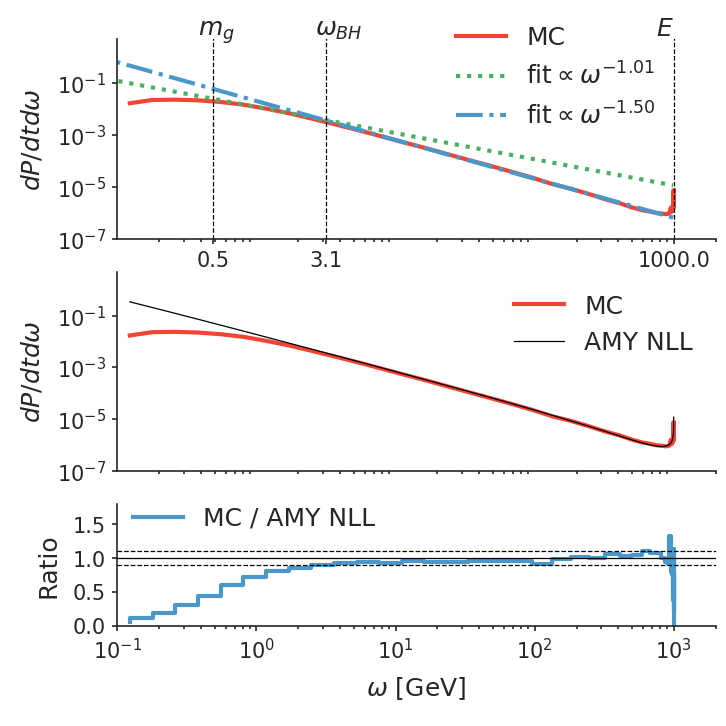
\includegraphics[width=\columnwidth]{spectrum.png}
\caption{Radiated gluon spectrum in an infinite medium from a quark of energy $E=500$ GeV, with a coupling constant $\alpha_s = 0.1$. The top frame shows the spectrum (red-dashed line) and power law fit (green-dotted and blue-dash-dotted lines) in different gluon energy ($0<\omega < E$) regions, separated by energy scales $m_g$, $\hat{q}_0\lambda_g^2 \sim 2\pi T$. The middle frame is the same calculation compared to the incoherent spectrum and the AMY semi-analytic result. The bottom frame is the ratio between the Monte-Carlo simulation and the semi-analytic calculation.}
\label{fig:spectrum}
\end{figure}

\begin{figure}
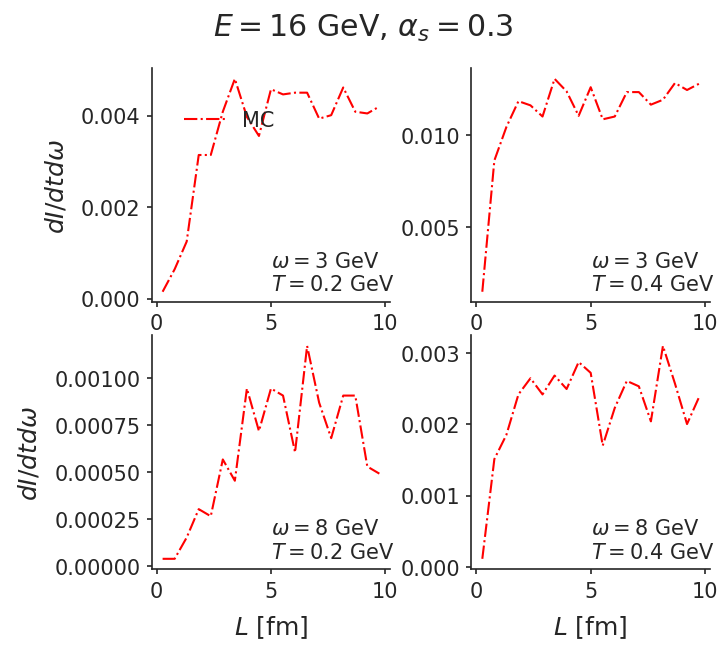
\includegraphics[width=\columnwidth]{spectrum_L.png}
\caption{Comparison of the path-length dependent energy-differential rate $dP/(dtd\omega)$ from the Monte-Carlo implementation using $\alpha_s = 0.3$ to the theoretical baseline calculation \cite{CaronHuot:2010bp}. The light quark energy is $16$ GeV.}
\label{fig:spectra-L-alphas=0.3}
\end{figure}

In an infinite static medium, the formula for the gluon radiation spectrum (we only use the one for a gluon splitting from a quark) is derived in \cite{Arnold:2002zm,Arnold:2003zc},
\begin{eqnarray}\label{eq:AMY-1}
\nonumber
\frac{dP_{q\rightarrow qg}}{dt dx} &=& \frac{1}{2E\nu_q} \frac{\alpha_s d_F P_{q\rightarrow qg}(x)}{2x^2(1-x)^2}\int\frac{d^2\vec{h}}{(2\pi)^2}2\vec{h}\cdot \mathfrak{Re} \vec{F} \\
&\times& [1+f_g(xp)][1-f_q((1-x)p)],
\end{eqnarray}
where $\vec{F}(\vec{h}; p, x)$ satisfies the following equation,
\begin{eqnarray}\label{eq:AMY-2}
\nonumber
2\vec{h} &=& i\frac{h^2 \vec{F}(\vec{h})}{p^3 2x(1-x)} \\
\nonumber
&+& g^2\int \frac{dq_\perp^2 \mathcal{A}(q_\perp^2)}{(2\pi)^2}\left\{\frac{C_A}{2}\left[\vec{F}(\vec{h}) - \vec{F}(\vec{h}+p\vec{q}_\perp)\right]\right. \\
\nonumber
&& \phantom{} + \left(C_F - \frac{C_A}{2}\right)\left[\vec{F}(\vec{h}) - \vec{F}(\vec{h}-xp\vec{q}_\perp)\right] \\
&& \phantom{sss} + \left. \frac{C_A}{2}\left[\vec{F}(\vec{h}) - \vec{F}(\vec{h}-(1-x)p\vec{q}_\perp)\right] \right\}.
\end{eqnarray}
The collision kernel of a gluon in a thermalized QGP is,
\begin{eqnarray}\label{eq:kernel}
\mathcal{A}(q_\perp^2) = \frac{T m_D^2}{q_\perp^2(q_\perp^2+m_D^2)}.
\end{eqnarray}
The exact solution can be obtained numerically, but the author of \cite{Arnold:2008zu} obtained a semi-analytic solution to next-to-leading-log ($[\ln(E/T)]^{-1}$) accuracy that is easier to use,
\begin{eqnarray}\label{eq:AMY-NLL}
\frac{dP_{q\rightarrow qg}^{\textrm{NLL}}}{dt dx} &=& \frac{\alpha_s P_{q\rightarrow qg}(x)}{2\pi}\frac{ \sqrt{2} d_F }{\nu_q }  \frac{m_D^2\hat{\mu}_\perp^2(x)}{2x(1-x)E}. 
\end{eqnarray}
Because we do not use quantum statistics in the Monte Carlo simulations, we have dropped the Bose enhancement and the Pauli blocking factors from the original formula.
The remaining terms are organized such that the last factor plays the role of the inverse formation time.
The dimensionless quantity $\hat{\mu}_\perp^2(x)$ is determined by the self-consistency condition,
\begin{eqnarray}\label{eq:AMY-sf}
\nonumber
\hat{\mu}_\perp^2 && = \frac{gT}{m_D} \sqrt{\frac{2x(1-x)E}{\pi T}}\left\{
\frac{C_A}{2}(1-x)^2\ln\left[\frac{\xi\hat{\mu}_\perp^2}{(1-x)^2}\right] + \right. \\
&&\left.\left(C_F-\frac{C_A}{2}\right)x^2\ln\left(\frac{\xi\hat{\mu}_\perp^2}{x^2}\right) + \frac{C_A}{2}\ln(\xi\hat{\mu}_\perp^2)\right\}^{\frac{1}{2}}.
\end{eqnarray}
$\xi\approx9.09916$ is a constant. 
The NLL result is a good approximation when $\ln(xE/T)$ is large. 
It rises above the numerical solutions with  when $\ln(xE/T)$ is small.
We are able to compensate for the deviation between the NLL approximation and the full numerical solution by including an additional multiplicative correction factor to Equation \ref{eq:AMY-NLL}, 
\begin{eqnarray}\label{eq:correction}
R_{\textrm{corr}} = \frac{1}{1+0.8\left(xE/T\right)^{-0.7}}.
\end{eqnarray}
It mimics the systematic deviation of Equation \ref{eq:AMY-NLL} from the numerical solution. 
Later we will see that this deviation is not significant for the relevant temperatures and parton energies larger than $10$ GeV.

To elucidate the physical interpretation of $\hat{\mu}_\perp^2$, we also quote the leading-log result from \cite{Arnold:2008zu} (terms reorganized),
\begin{eqnarray}\label{eq:AMY-LL}
\nonumber
\frac{m_D^2\hat{\mu}_{\perp, \textrm{LL}}^2}{2x(1-x)E} &=& 
\left(\frac{4C_A\alpha_s T m_D^2 \ln\left(Q_0^2/m_D^2\right)}{2x(1-x)E}\right)^{\frac{1}{2}}\\
&\times& \left(1-x+\frac{C_F}{C_A}x^2\right)^{\frac{1}{2}}
\end{eqnarray}
The logarithmic term comes from the integration of $q_\perp^2 A(q_\perp^2)dq_\perp^2$ that enters $\hat{q}$.
$Q_0^2$ is an estimated upper limits of the integration.
We see that the spectrum is proportional to $\sqrt{\hat{q}/\omega}$, corroborating the previous qualitative arguments.
The factor in the second line is included in the formation time redefinition in Equation \ref{eq:formation-time-def} of the ``modified rescattering" approach.
At the NLL order, $Q_0^2/m_D^2$ (equivalently $\hat{\mu}_\perp^2$) is improved by the self-consistent Equation \ref{eq:AMY-sf} that $Q_0^2/m_D^2 \sim \sqrt{\hat{q}\omega}/m_D^2\sim \tau_f\hat{q}/m_D^2$. 
This is corrected in the ``modified rescattering" approach by the $u$ factor in the acceptance. 
Of course, the form of correction is specific to the leading order collision kernel that has a long tail at large $q_\perp^2$.

For the case of a thin medium, a compact result is derived in \cite{Arnold:2009mr}. 
It already combines the contributions from a single-hard scattering and multiple-soft scatterings.
The energy loss reads,
\begin{eqnarray}\label{eq:dE-thin}
\Delta E = \pi C_F C_A N_0 \alpha_s^3 T^3 L^2 \ln\left(\frac{E}{m_D^2 L}\right).
\end{eqnarray}
The factor $N_0 = 6\zeta(3)(1+N_f/4)/\pi^2 \approx 1.28$ 
is obtained using quantum statistics for $N_f=3$. Since it is very close to the value calculated using classical statistics ($12/\pi^2 \approx 1.22, N_f=3$), we will not correct it in the comparison of the next section.

Next, we shall consider an expanding medium with a power law fall-off for the temperature: 
\begin{eqnarray}
T^3 = T_0^3\left(\frac{\tau_0}{\tau}\right)^{2-1/\nu}
\end{eqnarray}
The authors of \cite{Baier:1998yf} have calculated the radiation spectrum using the multiple-soft scattering approximation as,
\begin{eqnarray}
\frac{dP}{dx} &=& \frac{\alpha_s}{2\pi}P_{q\rightarrow qg}(x)\mathfrak{Re}\int_{\tau_0}^{\tau_0+L}\frac{dt_f}{t_f}\int_{\tau_0}^{t_f}\frac{dt_i}{t_i} \frac{1}{\nu^2}\\
\nonumber
&& \left.\left[ I_{\nu-1}(z_i)K_{\nu-1}(z_f)-I_{\nu-1}(z_f)K_{\nu-1}(z_i)\right]^{-2}\right|_{\omega}^{\omega=\infty},\\
z_{i,f} &=& 2i\nu \sqrt{\frac{\hat{q}_g(1-x+C_F/C_A x^2)}{2(1-x)\omega}} \tau_0 \left( \frac{t_{i,f}}{\tau_0}\right) ^{1/2\nu}
\end{eqnarray}
For $\nu=0.5$, this expression reduces to the static BDMPS result \cite{Baier:1996kr}. 
The Bjorken expansion $T \propto \tau^{-1/3}$ can be obtained by taking the limit $\nu \rightarrow 1$ \cite{PhysRevD.27.140}.
In an expanding medium, e.g. $\nu=1$, the transverse momentum broadening is,
\begin{equation}\label{eq:expanding-kt2}
\left\langle k_\perp^2\right\rangle \sim \int_{t_1}^{t_1+\tau_f
}\hat{q}(t)dt \sim \frac{t_1}{\tau_f}  \ln\left(1+\frac{\tau_f}{t_1}\right) \hat{q}(t_1)\tau_f
\end{equation}
So if the formation time is very short compared to the typical expansion time scale $d\ln(T)/d\tau \sim t_1$, the transverse broadening becomes $\left\langle k_\perp^2\right\rangle \sim \hat{q}(t_1)\tau_f$, which is the same as the one obtained in a static medium defined by the local temperature at $t_1$.
However, for large formation times, $\left\langle k_\perp^2\right\rangle$ becomes significantly smaller than the one determined using a local static medium.
We will come back to the impact of a local approximation in the next section. 
The BDMPS calculation assumes multiple-soft scatterings, so we only use it in a medium thick enough that
\begin{eqnarray}\label{eq:BDMPS-requrement}
\omega_c \sim \left\langle k_\perp^2 \right\rangle L > E.
\end{eqnarray}

We would like to remark that all of these analytic formulas are derived in the eikonal limit, so correspondingly in the Monte-Carlo simulations we reset the mother parton's four momentum back to its initial state after each time step and the gluon four-momentum is rescaled such that the energy is unchanged.



\section{results}\label{section:results}
In this section, we compare the outcome of the three different MC LPM implementations described in Section \ref{section:MC} to the theoretical reference outlined in Section \ref{section:Theo}. 
It is easier to compare the energy loss first, since it only depends on the integration over the spectrum and not on its details.
It will be shown that the ``modified rescattering" approach performs the best in comparison to the theory references. 
We will also validate its radiation spectrum.


In Figure \ref{fig:eloss-inf}, we show the calculation of energy loss per unit path length $dE/dx$ of a quark in an ``infinitely large" medium. 
Technically, $dE/dx$ is measured after an evolution time long enough ($L\gg L_c$) that finite size effects have faded away.
The results presented are normalized by $1/(\alpha_s^2 \sqrt{ET^3})$ in anticipation of the scaling $dE/dx \propto \alpha_s^2 \sqrt{ET^3}$.
For each column, we double the value of $\alpha_s$ and for each row, the temperature is increased by $0.2$ GeV. 
Within each subplot, the parton energy varies from $10$ GeV to $200$ GeV.
Different Monte Carlo implementations of the LPM effect are shown in colored lines, AMY NLL results are shown as black bands (we only integrate $\omega$ above the the Debye mass to calculate the AMY energy loss). 
The lower- and upper-bounds of the black bands correspond to the results with and without the correction factor in Equation \ref{eq:correction}.
We found that the ``modified rescattering" approach (red-dashed lines) reproduces the energy, temperature, and coupling constant dependence of AMY NLL energy loss very well.
There are actually two adjacent red-dashed lines in each subplot, corresponding to different choice of $\hat{t}_{\textrm{cut}}=m_D^2$ and $2 m_D^2$. 
The fact that the two lines are almost overlapping demonstrates the weak model dependence on this separation scale.
The ``coherence factor" approach (blue-dash-dotted lines) has a similar energy and temperature dependence to that of the theoretical baseline; however, it systematically deviates from the baseline for different values of the coupling constant in a logarithmic manner.
For the ``block radiation" approaches, the deviations from the baseline regarding their $\alpha_s$-dependence are even bigger and the energy dependence also gets worse, which is not surprising as we have discussed its shortcomings in Section \ref{section:MC}.

Next we examine the path-length ($L$) dependence of the energy loss $\Delta E$ of a quark with an initial energy of $E = 106$ GeV in a finite medium in Figure \ref{fig:eloss-ldep}.
Again, each column uses a different coupling constant and each row uses a different temperature. 
The path length within each subplot is varied up to four times $L_c^0$.
Here $L_c^0 = \sqrt{E/\hat{q}_0}$ with $\hat{q}_0 = C_A \alpha_s T m_D^2$ estimating the critical path length below which one expects a clear non-linear path-length dependence.
All three implementations show the non-linear increase of $\Delta E$ as function of $L$.
The ``modified rescattering" approach stays close to the theory calculations when $L<L_c^0$ for all cases, while the other two approaches deviate systematically as $\alpha_s$ is varied, similar to our previous findings for the energy-loss in the infinite matter case.

Now we go beyond comparing energy loss and directly validate the gluon emission spectrum using the ``modified rescattering" approach. 
The spectrum in an infinite medium $dP/dtd\omega$ is shown in Figure \ref{fig:spectrum} for a 500 GeV quark.
Please also refer to Appendix \ref{app:tune-spectrum} for a full comparison varying both the quark energy and the coupling constant.
The upper figure shows different domains of the emission spectrum separated by the gluon thermal mass $m_g$ and an estimate of the Bethe-Heitler energy $\lambda_g m_D^2 \sim 2\pi T$.
We have chosen $\alpha_s = 0.1$ so that the separation between $m_g$ and $2\pi T$ is more visible.
The spectrum with $\omega < m_g$ is suppressed due the use of a finite mass.
In the Bethe-Heitler region $m_g < \omega < 2\pi T$, incoherent $2\rightarrow 3$ processes described in Equation \ref{eq:GB-rate} dominate and the spectrum scales like $\omega^{-1}$.
In the LPM region $2\pi T < \omega < E$, the spectrum is dominated by coherent multiple scatterings and should be proportional to $\omega^{-3/2}$.
The power-law fits in each domain are very close to the expected scaling.
In the middle figure, we compare the above Monte-Carlo implementation to a calculation using the incoherent rate and to the AMY NLL approximation. 
Their ratios with respect to the MC implementation are shown in the bottom figure.
The ``modified rescattering" approach with $C_1 = 1$ and $C_2 = 1$ reproduces the incoherent limit with a gluon thermal mass for $\omega < 2\pi T$ and the LPM suppression for $\omega > 2\pi T$ within about $\pm 10\%$ accuracy.
In Figure \ref{fig:spectra-L-alphas=0.3}, the spectrum in a finite medium is compared to the full calculations from \cite{CaronHuot:2010bp}.
Using $\alpha_s = 0.3$, we have calculated the $L$-dependent gluon radiation rate of a 16 GeV quark.
The medium temperature of the left and the right columns are 0.2 GeV and 0.4 GeV respectively.
Top and bottom rows show the differential rates for the emitting gluon with $\omega = 3$ GeV and $\omega = 8$ GeV \footnote{to facilitate our analysis, we have selected events within a finite range $\omega\pm 0.5$ GeV}.
The radiation spectrum is recovered to a similar level of accuracy as in the infinite medium case.

\begin{figure}
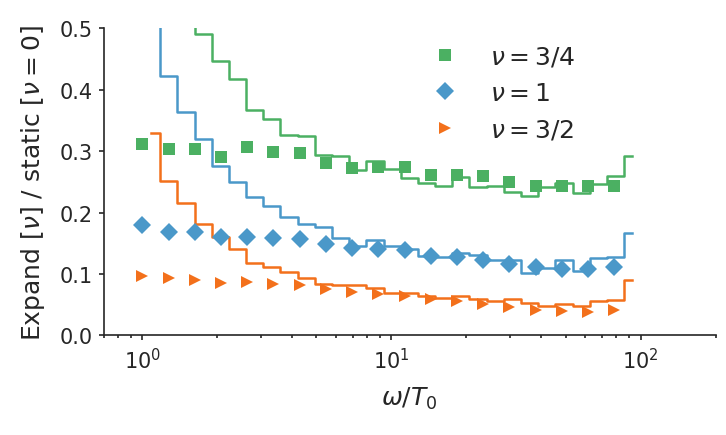
\includegraphics[width=\columnwidth]{spectrum_Bjorken.png}
\caption{The top frame shows the gluon radiation spectrum calculated with the the BDMPS formula (symbols) and Monte-Carlo simulations (lines) in a static medium ($\nu=1/2$), a slowly expanding medium ($\nu=5/7$) and a Bjorken expanding medium ($\nu\rightarrow 1$). In the bottom frame, we compute ratios of the analytic results and simulations between expanding cases and the static case. The parameters chosen are $\alpha_s=0.3$, $\tau_0 = 0.2$ fm/$c$, $L = 19.8$ fm/$c$, $T_0 = 1$ GeV.}
\label{fig:Bjorken-BDMPS}
\end{figure}

\begin{figure}
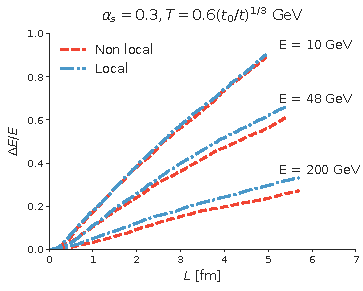
\includegraphics[width=\columnwidth]{Bjorken.pdf}
\caption{Energy loss fraction $\Delta E /E$ as function of path length $L$ for three different energies. Red-dashed lines are direct simulations (the non-local case) and blue-dash-dotted lines are results using the local approximation.}
\label{fig:Bjorken}
\end{figure}

Moving toward a comparison in an expanding medium, we perform a calculation using only the diffusion and the diffusion induced radiation  processes with the ``modified rescattering" LPM implementation, since this setup allows us to use the same $\hat{q}_g$ in both the BDMPS formula and the Monte-Carlo calculation.
For simplicity, we choose $\hat{q}_g = m_D^2 C_A\alpha_s T$ without the logarithmic term, thus the $u$ factor in the acceptance is not required. 
The expansion starts at $\tau_0=0.2$ fm/$c$ with $T_0=1$ GeV. 
The evolution stops at $\tau = 20$ fm/$c$. 
In Table \ref{tab:expand}, we listed three cases $\nu = 1/2, 5/7, 1$ corresponding to a static medium, a slowly expanding medium and a medium with Bjorken flow respectively.
In the third column, the power of the falling temperature as function of proper time is calculated. The last column lists the temperature at the end of the evolution.
We verify that for a 100 GeV quark and $\alpha_s = 0.3$, the requirement of Equation \ref{eq:BDMPS-requrement} is satisfied.
The top frame of Figure \ref{fig:Bjorken-BDMPS} directly compares the spectra to the theory baseline and the bottom frame shows the ratio between the expanding cases over the static case. 
The Monte-Carlo calculation performs very well in the LPM region, reflecting the decrease of induced radiation due to the dropping of temperature.
One also notice that the level of agreement decreases with increasing expansion rate. 
This is not a surprise, because the Monte-Carlo procedure described here is still not a fully quantum treatment.
\begin{center}
\begin{table}[h]
\caption{Expanding medium setup}\label{tab:expand}
\begin{tabularx}{\columnwidth}{XXXX}
\hline
Type & $\nu$ & $(2-1/\nu)/3$ & $T_f$ [GeV]\\ 
\hline
Static & 1/2 & 0 & 1.0\\
\hline
Slow & 5/7 & 1/5 & 0.40\\
\hline
Bjorken & $\rightarrow 1$ & 1/3 & 0.22\\
\hline
\end{tabularx} 
\end{table}
\end{center}

Finally, we revisit the validity of the local approximation briefly mentioned in the discussion following Equation \ref{eq:expanding-kt2}.
When the medium expansion rate is large compared to the inverse formation time, the following two scenarios are different,
\begin{itemize}
\item[1.]  {\it A non-local (direct) calculation}: radiated gluons are sensitive to the changing medium within the formation times.
\item[2.] {\it A local approximation}: calculated with rates obtained in the infinite medium defined by the local temperature at the radiation vertex.
\end{itemize} 
Here we study how well the local approximation performs for a typical coupling $\alpha_s = 0.3$.
The ``modified rescattering" approach is  a non-local calculation, because it performs gluon rescatterings at different space-time points during the lifetime of the "pre-formed gluons". 
To mimic the local approximation, we let each pre-formed gluon $i$ remember the temperature $T_i$ when it was first created and then perform rescatterings in a medium defined by that $T_i$.
The results are shown in Figure \ref{fig:Bjorken}. 
The difference between the two scenarios is negligible for $E=10$ GeV and  only moderate for a 200 GeV quark.
This is because for the coupling constant used, $\alpha_s = 0.3$, the ratio of the estimated maximum formation time $\sqrt{2x(1-x)E/\hat{q_0}}$ to the inverse temperature changing rate $(d\ln(T)/dt)^{-1}$,
\begin{eqnarray}
L_c \frac{d\ln(T)}{dt} = \sqrt{\frac{0.5 E}{6\pi C_A\alpha_s^2 T_0^3 9\tau\tau_0}} \approx \sqrt{\frac{0.7 \textrm{ fm}/c}{\tau_0+L}}
\end{eqnarray}
is not large after a few fm/$c$. 
However, in more realistic event-by-event hydrodynamics simulations, the temperature profiles are much more complicated.
Initial condition fluctuations create medium hot spots and the radial expansion boosts the fluid's local  rest frame.
We therefore consider it premature to conclude from this study utilizing Bjorken flow that the local approximation is also justified for more realistic event-by-event simulations.


\section{Running coupling and mass dependence}\label{section:disscuss}
\begin{figure}
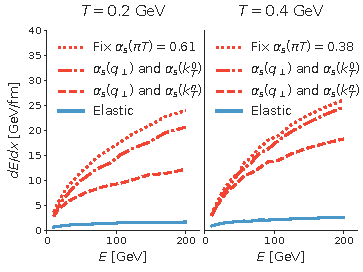
\includegraphics[width=\columnwidth]{Eloss_infinite_run.pdf}
\caption{Impact of the running of the coupling constant on the radiative energy loss. The dotted lines are calculated using a fixed coupling $\alpha_s(2\pi T)$ for reference. The dashed-dotted lines uses the prescription $\alpha_s^{\textrm{el}}(q_\perp)$ and $\alpha_s^{\textrm{rad}}(k_{\perp,0})$. The dashed lines further modify the radiation vertex with $\alpha_s^{\textrm{rad}}(k_{\perp,n})$.}
\label{fig:run}
\end{figure}
This section focus on improving our model by introducing a running coupling constant and mass effects. 
However, due to their complexity, we did not found applicable theory baseline results to compare to.
As a result, the proposed methods in this section should be considered as tentative.

We replace the fixed coupling by a running coupling constant  following the prescription described in \cite{Arnold:2008zu}.
This involves two changes in the formula. 
For elastic scattering vertices, $\alpha_s^{\textrm{el}}$ is evaluated at the $t$-channel momentum transfer squared. 
This is already the feature of {\tt Lido}.
For splitting vertices,  $\alpha_s^{\textrm{rad}}$ should be evaluated at the final gluon transverse momenta squared,
\begin{eqnarray}\label{eq:kTn}
k_{\perp,n}^2 = \left(\vec{k}_{\perp,0}+\vec{q}_1+\cdots+\vec{q}_n\right)^2.
\end{eqnarray} 
In the {\tt Lido} model, the original scale used for $\alpha_s^{\textrm{rad}}$ is $k_{\perp,0}^2$ from the $2\rightarrow 3$ process.
Therefore, we modify the acceptance probability $p$ to
\begin{eqnarray}
p' = \min\left\{1, u\frac{\tilde{\lambda}}{\tau_f}\frac{\alpha_s(k_{\perp,n})}{\alpha_s(k_{\perp,0})}\right\}.
\end{eqnarray}
The order of magnitude of $k_{\perp,n}^2$ is $\sqrt{\hat{q}\omega}$ and it is about $\sqrt{\omega/T}$ times larger than $k_{\perp,0}^2$ for gluons in the LPM region, therefore the running coupling effect suppresses the spectrum by another factor of $\alpha_s(k_{\perp,n})/\alpha_s(k_{\perp,0})$.
In Figure \ref{fig:run}, we show three calculations in a static medium. The dotted lines, as references, uses a fixed coupling constant evaluated at a thermal scale $\alpha_s = \alpha_s(2\pi T)$ .
This scale is also the lowest scale cut-off for the running coupling constant in our model \footnote{please see Appendix \ref{app:alphas} for details. Note that this minimum scale is not required in the original work \cite{Arnold:2008zu} where all scales are assumed to be much greater than $\Lambda_{\textrm{QCD}}$.}.
The dash-dotted lines are running coupling calculations where the $\alpha_s^{\textrm{el}}$ is evaluated at $\hat{t}$ and the $\alpha_s^{\textrm{rad}}$ at $k_{T,0}$.
The dashed lines are also running coupling calculations but evaluate $\alpha_s^{\textrm{rad}}$ at $k_{\perp,n}$ through the modified acceptance $p'$.
The running coupling effect results in a reduction of the energy loss compared to the fixed coupling references.

\begin{figure}
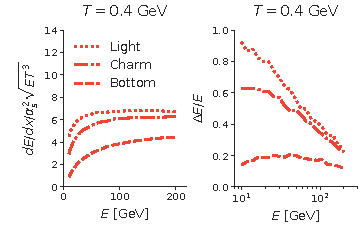
\includegraphics[width=\columnwidth]{Eloss_mass.pdf}
\caption{A demonstration of the mass effect with $\alpha_s=0.3$. Left frame: scaled energy loss rate in an infinite medium for light quarks, charm quarks and bottom quarks. Right frame: energy loss fraction of light quarks, charm quarks and bottom quarks at a path length $L=5$ fm.  }
\label{fig:mass}
\end{figure}

Finally, we include quark mass dependencies in our calculation in order to expand our LPM treatment to heavy quarks. These include the massive particle kinematics, a substitution in the formation time,
\begin{eqnarray}
(1-x)m_g^2 \rightarrow x^2M^2 + (1-x)m_g^2
\end{eqnarray}
and the so-called ``dead-cone" effect that suppresses collinear radiations with angles $\theta \sim k_\perp/k < M/E$. 
The massive version of the $2\rightarrow3$ improved Gunion-Bertsch matrix-element has been derived in \cite{Uphoff:2014hza}.
If we simply replace the matrix-element with the massive one, the dead cone suppression involves the factor,
\begin{eqnarray}
\frac{k_{\perp,0}^2}{k_{\perp,0}^2+x^2M^2}
\end{eqnarray}
However, because rescatterings continue to increase the average $k_{\perp}^2$ , the factor is different by the time the gluon is formed,
\begin{eqnarray}
\frac{k_{\perp,n}^2}{k_{\perp,n}^2+x^2M^2}.
\end{eqnarray}
The solution is to use the $2\rightarrow3$ matrix-element without mass effect to generate pre-formed gluons, while implementing the dead-cone suppression by adding another factor to the acceptance,
\begin{eqnarray}
p'' = \min\left\{1, u\frac{\tilde{\lambda}}{\tau_f}\frac{\alpha_s(k_{\perp,n})}{\alpha_s(k_{\perp,0})} \left[\frac{k_{\perp,n}^2}{k_{\perp,n}^2+x^2 M^2}\right]^4\right\}.
\end{eqnarray}
On the left of Figure \ref{fig:mass}, the scaled energy loss rate in an infinite medium is extracted from simulations for light (massless), charm ($M=1.3$ GeV) and bottom ($M=4.2$ GeV) quarks. 
On the right, it is the energy loss fraction at a fixed path-length $L=5$ fm.
In both cases, the mass introduces the energy loss ordering, $\Delta E_{\textrm{light}} > \Delta E_c > \Delta E_b$ and the differences decrease at higher energy.

%\begin{figure*}
%\includegraphics[width=\textwidth]{raa_mclpm.pdf}
%\caption{This figure shows what is predicted for D-meson observables at the leading order level considering running coupling and mass effect. The only parameter is the minimum scale in the running $\alpha_s(\max\{Q,\mu\})$. The solid lines use $\mu = 2\pi T$ and the dashed lines use $\mu=\pi T$}
%\end{figure*}


\section{Summary and outlook}\label{section:summary}


We have studied three different Monte-Carlo implementations of the LPM suppression of jet energy-loss and have compared them to a theory baseline.
We have shown that the ``modified rescattering" approach reproduces the coupling constant, temperature, parton energy and path-length dependences of the theoretical baselines for both infinite- and thin-medium limits.
The overall level of agreement between the simulated radiation spectrum and theory is promising given the simplicity and limits of a Monte-Carlo procedure. Tentative running coupling and dead-cone effect dependencies have also implemented.
This work allows us to reduce the theory uncertainty introduced in the numerical implementation of the perturbative QCD transport of hard partons inside a quark-gluon plasma, which is instrumental for performing an unambiguous examination of theory assumptions and a more meaningful phenomenological extraction of jet and heavy quark transport properties in a model-to-data comparison.
Moreover, a Monte-Carlo generator that is tuned to match leading order theory calculation will serve as a promising starting point to implement next-to-leading-order effects in the phenomenology model.


\begin{acknowledgments}
SAB, WK and YX are supported by the U.S. Department of Energy Grant no. DE-FG02-05ER41367. WK is also supported by NSF grant OAC-1550225.
\end{acknowledgments}

\begin{appendices}
\section{Running coupling constant}\label{app:alphas}
The leading order running couplings constant with three quark flavors is
\begin{eqnarray}
\alpha_s(Q) = \frac{4\pi}{9\log(Q^2/\Lambda_{\textrm{QCD}}^2)},
\end{eqnarray}
and $\Lambda_{\textrm{QCD}} = 0.2$ GeV. In a medium, we require that the scale of a process cannot be arbitrarily small compared to the temperature. The resulting $Q$ is cut off at a medium scale defined by $\mu\pi T$ ($\mu=2$ by default) and $\alpha_s(Q) = \alpha_s(\max\{Q,\mu\pi T\})$. We treat $\mu$ as a parameter of the model. It is also a major source of uncertainty in the predictions. In fact for a typical $T=0.3$ GeV, $\alpha_s(\pi T \sim 4\pi T)$ varies from 0.45 to 0.24.

\begin{figure}
\includegraphics[width=\columnwidth]{spectrum_E_alpha0d1.png}
\caption{Ratios of Monte-Carlo calculated gluon emission spectra to the AMY NLL spectra (gray bands) and to the Gunion-Bertsch incoherent spectra (blue lines), using $\alpha_s = 0.1$. The quark energies are $E$ is 10, 50, 100, and 500 GeV as indicated by the rightmost vertical dashed lines in each subplot. The horizontal dashed lines denote $\pm 10\%$ deviation from unity.}
\label{fig:spectra-alphas=0.1}
\end{figure}


\begin{figure}
\includegraphics[width=\columnwidth]{spectrum_E_alpha0d3.png}
\caption{The same as Figure \ref{fig:spectra-alphas=0.1}, but for $\alpha_s = 0.3$.}
\label{fig:spectra-alphas=0.3}
\end{figure}

\section{Gunion-Bertsch rate under soft transverse momenta exchange}
\label{app:consistency}
The Gunion-Bertsch matrix-element factorizes the $2\rightarrow3$ process into the product of a $2\rightarrow2$ process and the radiative $1\rightarrow 2$ process. 
In the vacuum, this is,
\begin{eqnarray}
|M_{\textrm{GB}}|^2 &=& |M_{2\rightarrow 2}|^2 16 C_A \pi \alpha_s \frac{(1-\bar{x})^2q_\perp^2}{k_\perp^2\left(\vec{q}_\perp-\vec{k}_\perp\right)^2}.
\end{eqnarray}
In medium, a gluon thermal mass regulates the divergence. 
For hard splitting where $k_\perp \gg q_\perp \sim m_D$, 
\begin{eqnarray}
|M_{\textrm{GB}}|^2 &\approx & q_\perp^2 |M_{2\rightarrow 2}|^2 16 C_A \pi \alpha_s \frac{(1-\bar{x})^2}{k_\perp^4}.
\end{eqnarray}
Using this approximation in the scattering rate Equation \ref{eq:GB-rate} and factorizing the $q_\perp$ and $k_\perp$ integrations yields,
\begin{eqnarray}
\Gamma &=& \frac{1}{2E_1}\int\frac{f_i(p_2)d\vec{p_2}^3}{(2\pi)^3 2p_2}2\hat{s} \frac{d\sigma_{2\rightarrow 2}}{d\hat{t}}q_\perp^2 d\hat{t} \nonumber \\
&\times& \int 16\pi C_A \alpha_s \frac{(1-\bar{x})^2}{k_\perp^4} \frac{d\vec{k}^3}{(2\pi)^3 2k}
\end{eqnarray}
For the case of a quark, the first integration over the $2\rightarrow 2$ cross-section gives $C_F/C_A\hat{q}_g$, after summing over the degeneracy of the gluonic and the fermionic scattering centers.
Rewriting the second $k$ integration in terms of $x, k_\perp^2$ in the limit $\bar{x}\ll 1$, the rate becomes,
\begin{eqnarray}\label{eq:GB-LGV}
\Gamma &=& \hat{q}_g \int \frac{\alpha_s C_F}{\pi} \frac{dk_\perp^2}{k_\perp^4} \frac{dx}{x}
\end{eqnarray}
Finally, inserting the coherence factor of Equation \ref{eq:GB-rate-LPM}, the gluon radiation rate becomes identical to the one used in \cite{Cao:2013ita} when $x\ll 1$.
After reorganizing the incoherent rate Equation \ref{eq:GB-LGV} and performing the $k_\perp$ integration with the regulator $m_g$, we obtain,
\begin{eqnarray}
\Gamma &=& \int \frac{\alpha_s}{\pi} \frac{C_F}{x}dx \frac{\hat{q}_g}{m_g^2} 
\end{eqnarray}
The factor $\frac{\hat{q}_g}{m_g^2}$ motivates our definition of the effective mean-free-path in Equation \ref{eq:effmpf}.

To estimate the order-of-magnitude of $\Delta t$ in the coherence factor, we apply the condition \ref{eq:delta-t-1} and the above approximated formula yields,
\begin{eqnarray}
\nonumber
1 &\sim& \alpha_s\hat{q}\Delta t \int_{\omega_{\min}}^{E} \frac{d\omega}{\omega}  \frac{dk_\perp^2}{k_\perp^4}  \left[1-\frac{\sin(\Delta t k_\perp^2/2\omega)}{\Delta t k_\perp^2/2\omega}\right]\\
\nonumber
&=& \alpha_s\hat{q}\Delta t^2 \int \frac{d\omega}{2\omega^2}  \int d\frac{2\omega}{\Delta t k_\perp^2}  \left[1-\frac{\sin(\Delta t k_\perp^2/2\omega)}{\Delta t k_\perp^2/2\omega}\right]\\
&=& \alpha_s\hat{q}\Delta t^3 \int \frac{d(\omega\Delta t)}{2(\omega\Delta t) ^2} f(2\omega\Delta t)
\end{eqnarray}
The limiting behavior of function $f(x)$ can be captured by a simple interpolation $Ax/(B+x)$.
Using this simple approximated form of $f(x)$, we conclude that the last integration has a logarithmic dependence on $E$, $\Delta t$, and the infrared cut-off $\omega_{\min}$.
Negelecting the logarithmic term, the order of magnitude of a typical $\Delta t$ is $(\alpha_s\hat{q})^{-1/3}\sim 1/\alpha_s T$.


\section{Energy and coupling constant dependence of radiation spectra}\label{app:tune-spectrum}
It is important to be aware of the known discrepancies between the Monte-Carlo implementation and the theory baseline, particularly if one investigates an observable that is sensitive to the details of the radiation spectra. 
In this appendix, we provide comparisons of radiation spectra at different values of energy and coupling constant for the reader's references.
Figure \ref{fig:spectra-alphas=0.1} and Figure \ref{fig:spectra-alphas=0.3} shows calculation using $\alpha_s = 0.1$ and $0.3$.
Within in each figure, different subplots vary the quark energy.
The gray bands are the ratios between the simulations and the AMY-NLL results (plotted for $\pi T < \omega < E$) and the blue lines are the ratios between the full simulations and the incoherent simulations (the Gunion-Bertsch rate, plotted for $0.1$ GeV $< \omega < 4\pi T $).
We notice that there are residual systematic discrepancies, but the overall difference is controlled within $\pm 15\%$ for the coupling constants, temperatures and energies under consideration.


\end{appendices}
\bibliography{mclpm} 
\end{document}
